

\chapter{Modeling Time-to-Event Outcomes}
 \label{chapter::survival-analysis}


\section{Examples}
Time-to-event data are common in biomedical and social sciences. Statistical analysis of time-to-event data is called
{\it survival analysis} in biostatistics and {\it duration analysis} in econometrics.
The former name comes from biomedical applications where the outcome
denotes the survival time or the time to the recurrence of the disease of interest. The
latter name comes from the economic applications where the outcome
denotes the weeks unemployed or days until the next arrest after being released from incarceration. See \citet{kalbfleisch2011statistical} for biomedical applications and \citet{heckman1984econometric} for economic applications. \citet{freedman2008survival} gave a concise and critical introduction to survival analysis. 



\subsection{Survival analysis}

The Combined Pharmacotherapies and Behavioral Interventions study evaluated the efficacy of medication, behavioral therapy, and their combination for the treatment of alcohol dependence \citep{anton2006combined}. Between January 2001 and January 2004, $n=1224$ recently alcohol-abstinent volunteers were randomized to receive medical management with 16 weeks of naltrexone (100mg daily) or placebo, with or without a combined behavioral intervention. It was a $2\times 2$ factorial experiment. The outcome of interest is the time to the first day of heavy drinking and other endpoints. I adopt the data from \citet{lin2016simultaneous}. 

\begin{lstlisting}
> COMBINE = read.table("combine_data.txt", header = TRUE)[, -1]
> head(COMBINE)
  AGE GENDER    T0_PDA NALTREXONE THERAPY   site relapse futime
1  31   male  3.333333          1       0 site_0       0    112
2  41 female 16.666667          1       1 site_0       1      8
3  44   male 73.333333          0       1 site_0       1     20
4  65   male 10.000000          1       0 site_0       0    112
5  39   male  0.000000          0       1 site_0       1      4
6  56   male 13.333333          0       0 site_0       1      1
\end{lstlisting}

\ri{NALTREXONE} and \ri{THERAPY} are two treatment indicators. \ri{futime} is the follow-up time, which is censored if \ri{relapse} equals 0. For those censored observations, \ri{futime} equals 112, so it is administrative censoring. Figure \ref{fig::histogram_combine_lindata} shows the histograms of \ri{futime} in four treatment groups. A large number of patients have censored outcomes. 
Other variables are covariates. 


\begin{figure}[th]
\centering
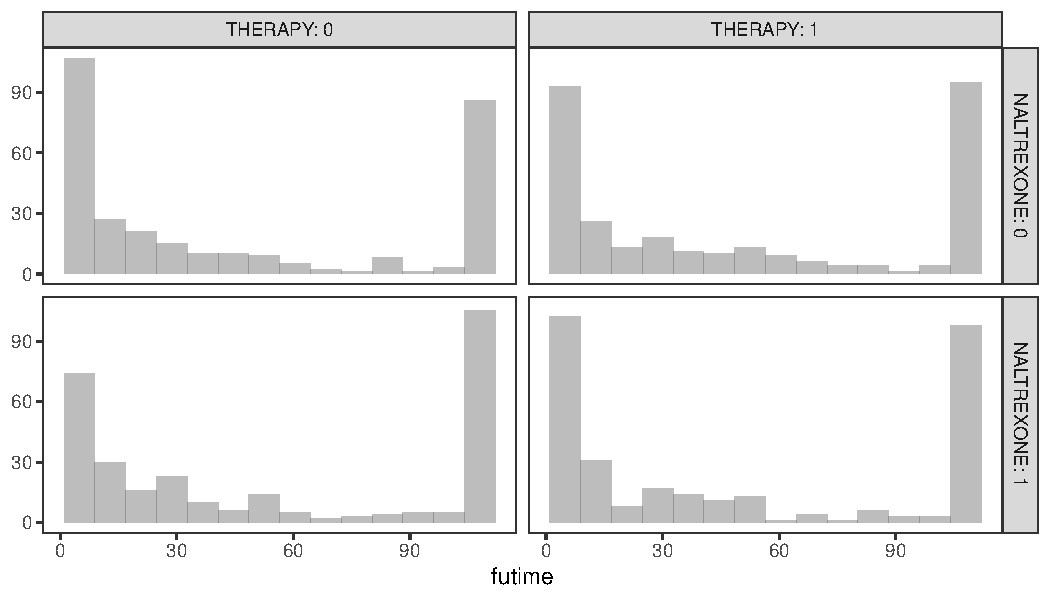
\includegraphics[width = \textwidth]{figures/combine_histograms.pdf}
\caption{Histograms of the time to event in the data from \citet{lin2016simultaneous}}\label{fig::histogram_combine_lindata}
\end{figure}



\subsection{Duration analysis}

\citet{carpenter2002groups} asked the question: Why does the U.S. Food and Drug Administration approve some drugs more quickly than others? With data about 450 drugs reviewed from 1977 to 2000, he studied the dependence of review times on various covariates, including political influence, wealth of the richest organization representing the disease, media coverage, etc. I use the version of data analyzed by
\citet{keele2010proportionally}. 
The outcome \ri{acttime} is censored indicated by \ri{censor}.
The original paper contains more detailed explanations of the variables. 


\begin{lstlisting}
> fda <- read.dta("fda.dta")
> names(fda)
 [1] "acttime"  "censor"   "hcomm"    "hfloor"   "scomm"   
 [6] "sfloor"   "prespart" "demhsmaj" "demsnmaj" "orderent"
[11] "stafcder" "prevgenx" "lethal"   "deathrt1" "hosp01"  
[16] "hospdisc" "hhosleng" "acutediz" "orphdum"  "mandiz01"
[21] "femdiz01" "peddiz01" "natreg"   "natregsq" "wpnoavg3"
[26] "vandavg3" "condavg3" "_st"      "_d"       "_t"      
[31] "_t0"      "caseid"  
\end{lstlisting}


An obvious feature of time-to-event data is that the outcome is non-negative. This can be easily dealt with by the log transformation. However, the outcomes may be censored, resulting in inadequate tail information. With right censoring, modeling the mean involves extrapolation in the right tail.  


\section{Time-to-event data}


Let $T\geq0$ denote the outcome of interest. We can characterize
a non-negative continuous $T$ using its density $f(t)$, distribution
function $F(t)$, survival function $S(t)=1-F(t)=\pr(T>t)$, and hazard
function
\[
\lambda(t)=\lim_{\Delta t\downarrow0}\pr(t\leq T<t+\Delta t\mid T\geq t)/\Delta t.
\]
Within a small time interval $[t,t+\Delta t]$, we have approximation
\[
\pr(t\leq T<t+\Delta t\mid T\geq t)\cong\lambda(t)\Delta t,
\]
so the hazard function denotes the death rate within a small interval conditioning on surviving up to time $t$.
Both the survival and hazard functions are commonly used to describe a positive random
variable. 
First, the survival function has a simple relationship with the expectation.

\begin{proposition}\label{prop::survival-mean}
For a non-negative random variable $T$,
$$
E(T) = \int_{0}^{\infty} S(t) \d t .
$$
\end{proposition}

Proposition \ref{prop::survival-mean} holds for both continuous and discrete non-negative random variables.
It states that the expectation of a nonnegative random variable equals the area under the survival function. It does not require the existence of the density function of $T$. 

\begin{myproof}{Proposition}{\ref{prop::survival-mean}}
Fubini's theorem allows us to swap the expectation and integral below:
\begin{eqnarray*}
E(T) &=& E \left\{  \int_0^{T}  \d t \right\}  \\
&=& E \left\{  \int_0^{\infty} 1(T > t) \d t \right\}  \\
&=&  \int_0^{\infty} E\{ 1(T > t)\}  \d t \\
&=& \int_0^{\infty} \pr (T > t)  \d t \\
&=& \int_{0}^{\infty} S(t) \d t .
\end{eqnarray*}
\end{myproof}

Second, the survival and hazard functions can determine each other in the following way.

\begin{proposition}\label{prop::hazard-pdf-survival}
For a non-negative continuous random variable $T$, 
\begin{align*}
\lambda(t) & =\frac{f(t)}{S(t)} = -\frac{\d}{\d t}\log S(t),\\
S(t) & =\exp\left\{ -\int_{0}^{t}\lambda(s)\d s\right\} .
\end{align*}
\end{proposition}



\begin{myproof}{Proposition}{\ref{prop::hazard-pdf-survival}}
By definition,
\begin{eqnarray*}
\lambda(t) &=&\lim_{\Delta t\downarrow0}\frac{\pr(t\leq T<t+\Delta t)}{\Delta t}\frac{1}{\pr(T\geq t)}  \\
&=&\lim_{\Delta t\downarrow0}\frac{F(t+\Delta t)-F(t)}{\Delta t}\frac{1}{S(t)}\\
&=&\frac{f(t)}{S(t)}.
\end{eqnarray*}
We can further write the above equation as
\begin{eqnarray*}
\lambda(t)  &=& \frac{f(t)}{S(t)} \\
&=& -\frac{\d S(t)/\d t}{S(t)} \\
&=&  -\frac{\d}{\d t}\log S(t),
\end{eqnarray*}
so we can use the Newton--Leibniz formula to obtain
\[
\d\log S(t)=-\lambda(t)\d t
\]
which implies
\[
\log S(t) - \log S(0)=-\int_{0}^{t}\lambda(s)\d s . 
\]
Because $\log S(0)=0$, we have $\log S(t) = -\int_{0}^{t}\lambda(s)\d s$, giving the final result. 
\end{myproof}


\begin{example}
[Exponential]
The Exponential$(\lambda)$ random variable $T$ has density $f(t) = \lambda e^{-\lambda t}$, survival function $S(t) = e^{-\lambda t}$, and constant hazard function
$
\lambda(t)= \lambda.
$
An important feature of the Exponential random variable is its memoryless property as shown in Proposition \ref{prop::memoryless}. 
%$$
%\pr(T \geq t+c \mid T\geq c) = \frac{  \pr(T \geq t+c) }{ \pr(T \geq c) } 
%= \frac{e^{-\lambda (t + c)}}{ e^{-\lambda c} } = e^{-\lambda t} = \pr(T \geq t),
%$$
%that is, the probability of surviving another $t$ time is always the same no matter how long the existing survival time is. 
\end{example}



\begin{example}
[Gamma]
The Gamma$(\alpha, \beta)$ random variable $T$ has density 
$
f(t) =   \beta^\alpha t^{\alpha-1} e^{-\beta t}/ \Gamma(\alpha). 
$
When $\alpha = 1$, it reduces to Exponential$(\beta)$ with a constant hazard function. In general, the survival function and hazard function do not have simple forms, but we can use \ri{dgamma} and \ri{pgamma} to compute them numerically. The left panel of Figure \ref{fig::gamma-lnorm-hazard-functions} plots the hazard functions of Gamma$(\alpha, \beta)$. When $\alpha <1$, the hazard function is decreasing; when $\alpha >1$, the hazard function is increasing. 
\end{example}



\begin{figure}
\centering
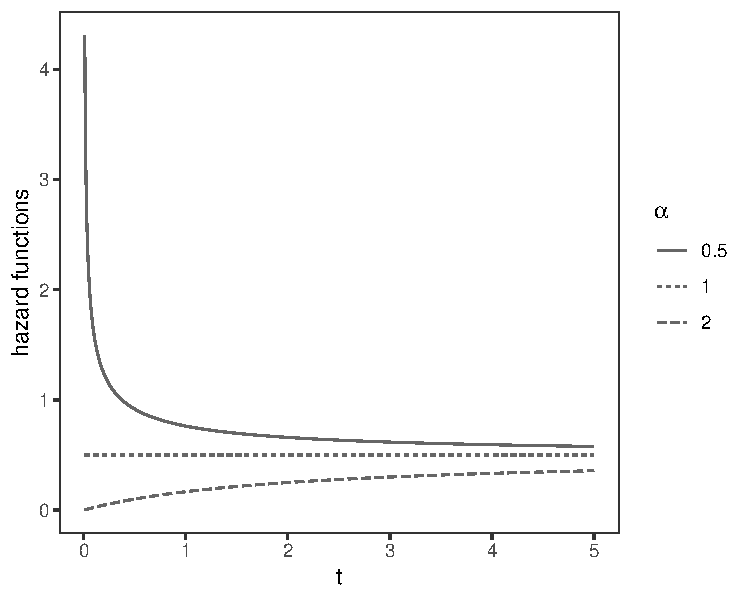
\includegraphics[width = 0.49\textwidth]{figures/gamma_hazard.pdf}
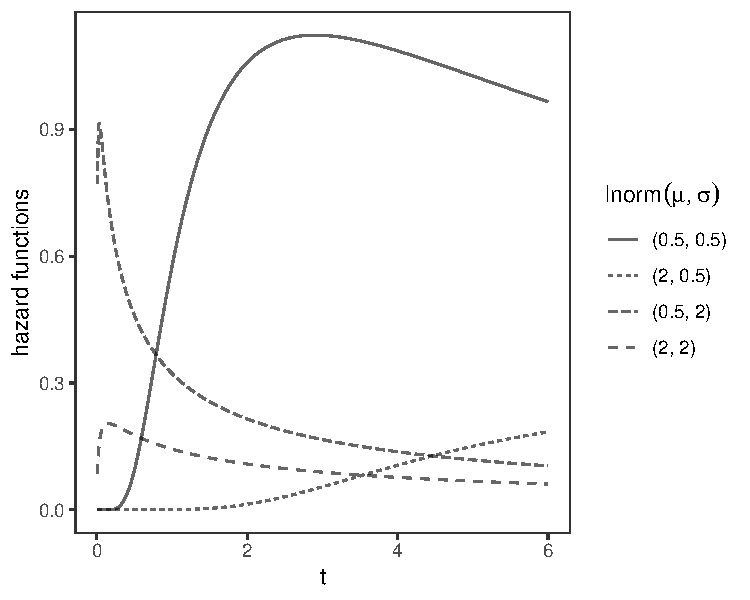
\includegraphics[width = 0.49\textwidth]{figures/lognormal_hazard.pdf}
\caption{Left: Gamma$(\alpha, \beta = 2)$ hazard functions; Right: Log-Normal$(\mu,\sigma^2)$ hazard functions}\label{fig::gamma-lnorm-hazard-functions}
\end{figure}





\begin{example}
[Log-Normal]
The Log-Normal random variable $T \sim $Log-Normal$(\mu,\sigma^2)$ equals exponential of $\N(\mu,\sigma^2)$. The right panel of Figure \ref{fig::gamma-lnorm-hazard-functions} plots the hazard functions with four different parameter combinations. 
\end{example}



\begin{example}
[Weibull]
The Weibull distribution has many different parametrizations. Here I follow the \ri{R} function \ri{dweibull}, which has a \ri{shape} parameter $a>0$ and \ri{scale} parameter $b>0$. The Weibull$(a,b)$ random variable $T$ can be generated by
\begin{eqnarray}
\label{eq::weibull-representation}
T = b Z^{1/a}
\end{eqnarray}
which is equivalent to
\[
\log T = \log b + a^{-1} \log Z,
\]
where $Z\sim $ Exponential$(1)$. We can verify that  $T$ has the density function
\[
f(t)=  \frac{a}{b} \left(  \frac{t}{b}   \right)^{a-1} \exp\left\{  - \left(  \frac{t}{b}   \right)^a \right\},
\]
survival function
$$
S(t)  = \exp\left\{  - \left(  \frac{t}{b}   \right)^a \right\},
$$
and hazard function
$$
\lambda(t) = \frac{a}{b} \left(  \frac{t}{b}   \right)^{a-1}.
$$
So when $a=1$, Weibull reduces to Exponential with constant hazard function. When $a>1$, the hazard function increases; when $a<1$, the hazard function decreases. 
\end{example}
 



We can characterize a positive discrete  random variable $T\in\left\{ t_{1},t_{2},\ldots\right\} $
by its probability mass function $f(t_{k})=\pr(T=t_{k})$, distribution
function $F(t)=\sum_{k:t_{k}\leq t}f(t_{k})$, survival function $S(t)=\sum_{k:t_{k}>t}f(t_{k})$,
and discrete hazard function
\[
\lambda_{k}=\pr(T=t_{k}\mid T\geq t_{k})=\frac{f(t_{k})}{S(t_{k}-)},
\]
where $S(t_{k}-)$ denotes the left limit of the function $S(t)$
at $t_{k}$. Figure \ref{fig::discrete-survival-fn} shows an example of a survival function for a discrete random variable, which shows that $S(t)$ is a step function and right-continuous with left limits. 


\begin{figure}
\centering
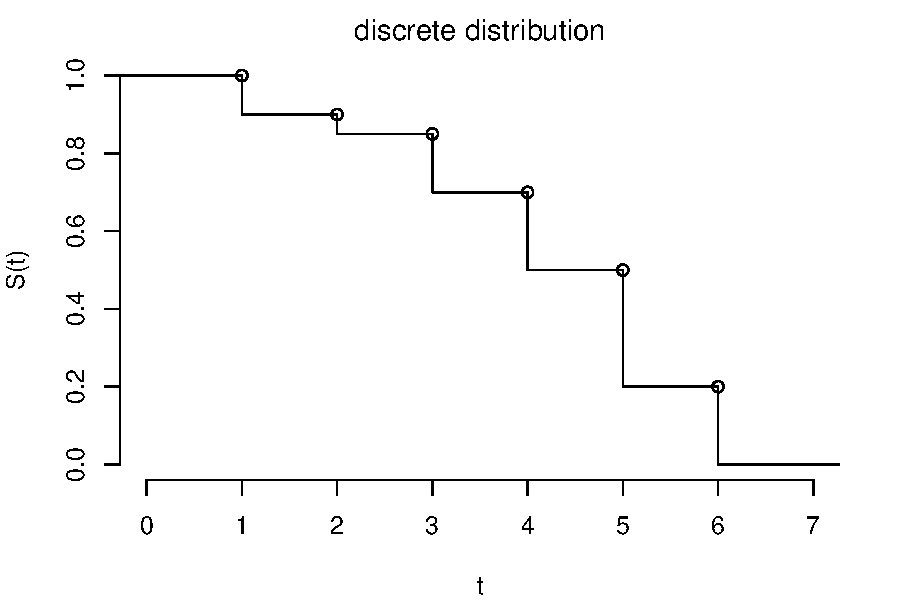
\includegraphics[width=0.9\textwidth]{figures/discrete_survival_fn.pdf}
\caption{Discrete survival function with masses $(0.1, 0.05, 0.15, 0.2, 0.3, 0.2)$ at $(1,2,3,4,5,6)$}
\label{fig::discrete-survival-fn}
\end{figure}
 


The discrete hazard and survival functions have the following
connection which will be useful for the next section. 


\begin{proposition}
\label{proposition:discrete-hazard}For a positive discrete random variable
$T$, its survival function is a step function determined by
\[
S(t)=\pr(T>t)=\prod_{k:t_{k}\leq t}(1-\lambda_{k}).
\]
\end{proposition}


Note that $S(t)$ is a step function decreasing at each $t_k$ because $\lambda_k$ is probability and thus bounded between zero and one. 


\begin{myproof}{Proposition}{\ref{proposition:discrete-hazard}}
By definition, 
\[
1-\lambda_{k}=1 - \pr(T=t_{k}\mid T\geq t_{k})=\pr(T>t_{k}\mid T\geq t_{k})
\]
is the probability of surviving longer than $t_{k}$ conditional on
surviving at least as long as $t_{k}$. We can verify Proposition
\ref{proposition:discrete-hazard} within each interval of the $t_{k}$'s.
For example, if $t<t_{1}$, then $S(t)=\pr(T>t)=1$; if $t_{1}\leq t<t_{2}$,
then 
\begin{eqnarray*}
S(t) &=&\pr(T>t_{1}) \\
&=& \pr(T>t_{1}, T\geq t_{1}) \\
&=&\pr(T>t_{1}\mid T\geq t_{1}) \pr(T\geq t_{1}) \\
&=&1-\lambda_{1};
\end{eqnarray*}
if $t_{2}\leq t<t_{3}$, then 
\begin{eqnarray*}
S(t) &=&\pr(T>t_{2})=\pr(T>t_{2}, T \geq t_{2}) \\
&=&\pr(T>t_{2}\mid T\geq t_{2})\pr(T\geq t_2)\\
&=&(1-\lambda_{2})(1-\lambda_{1}).
\end{eqnarray*}
We can also verify other values of $S(t)$ by induction. 
\end{myproof}
%

\section{Kaplan--Meier survival curve}


Without censoring, estimating the CDF or the survival function is rather straightforward. With IID data $(T_1, \ldots, T_n)$, we can estimate the CDF by $\hat{F}(t) =  n^{-1} \sumn 1(T_i \leq t) $ and the survival function by $\hat{S}(t) = 1 - \hat{F}(t)$. 




\begin{figure}
\centering
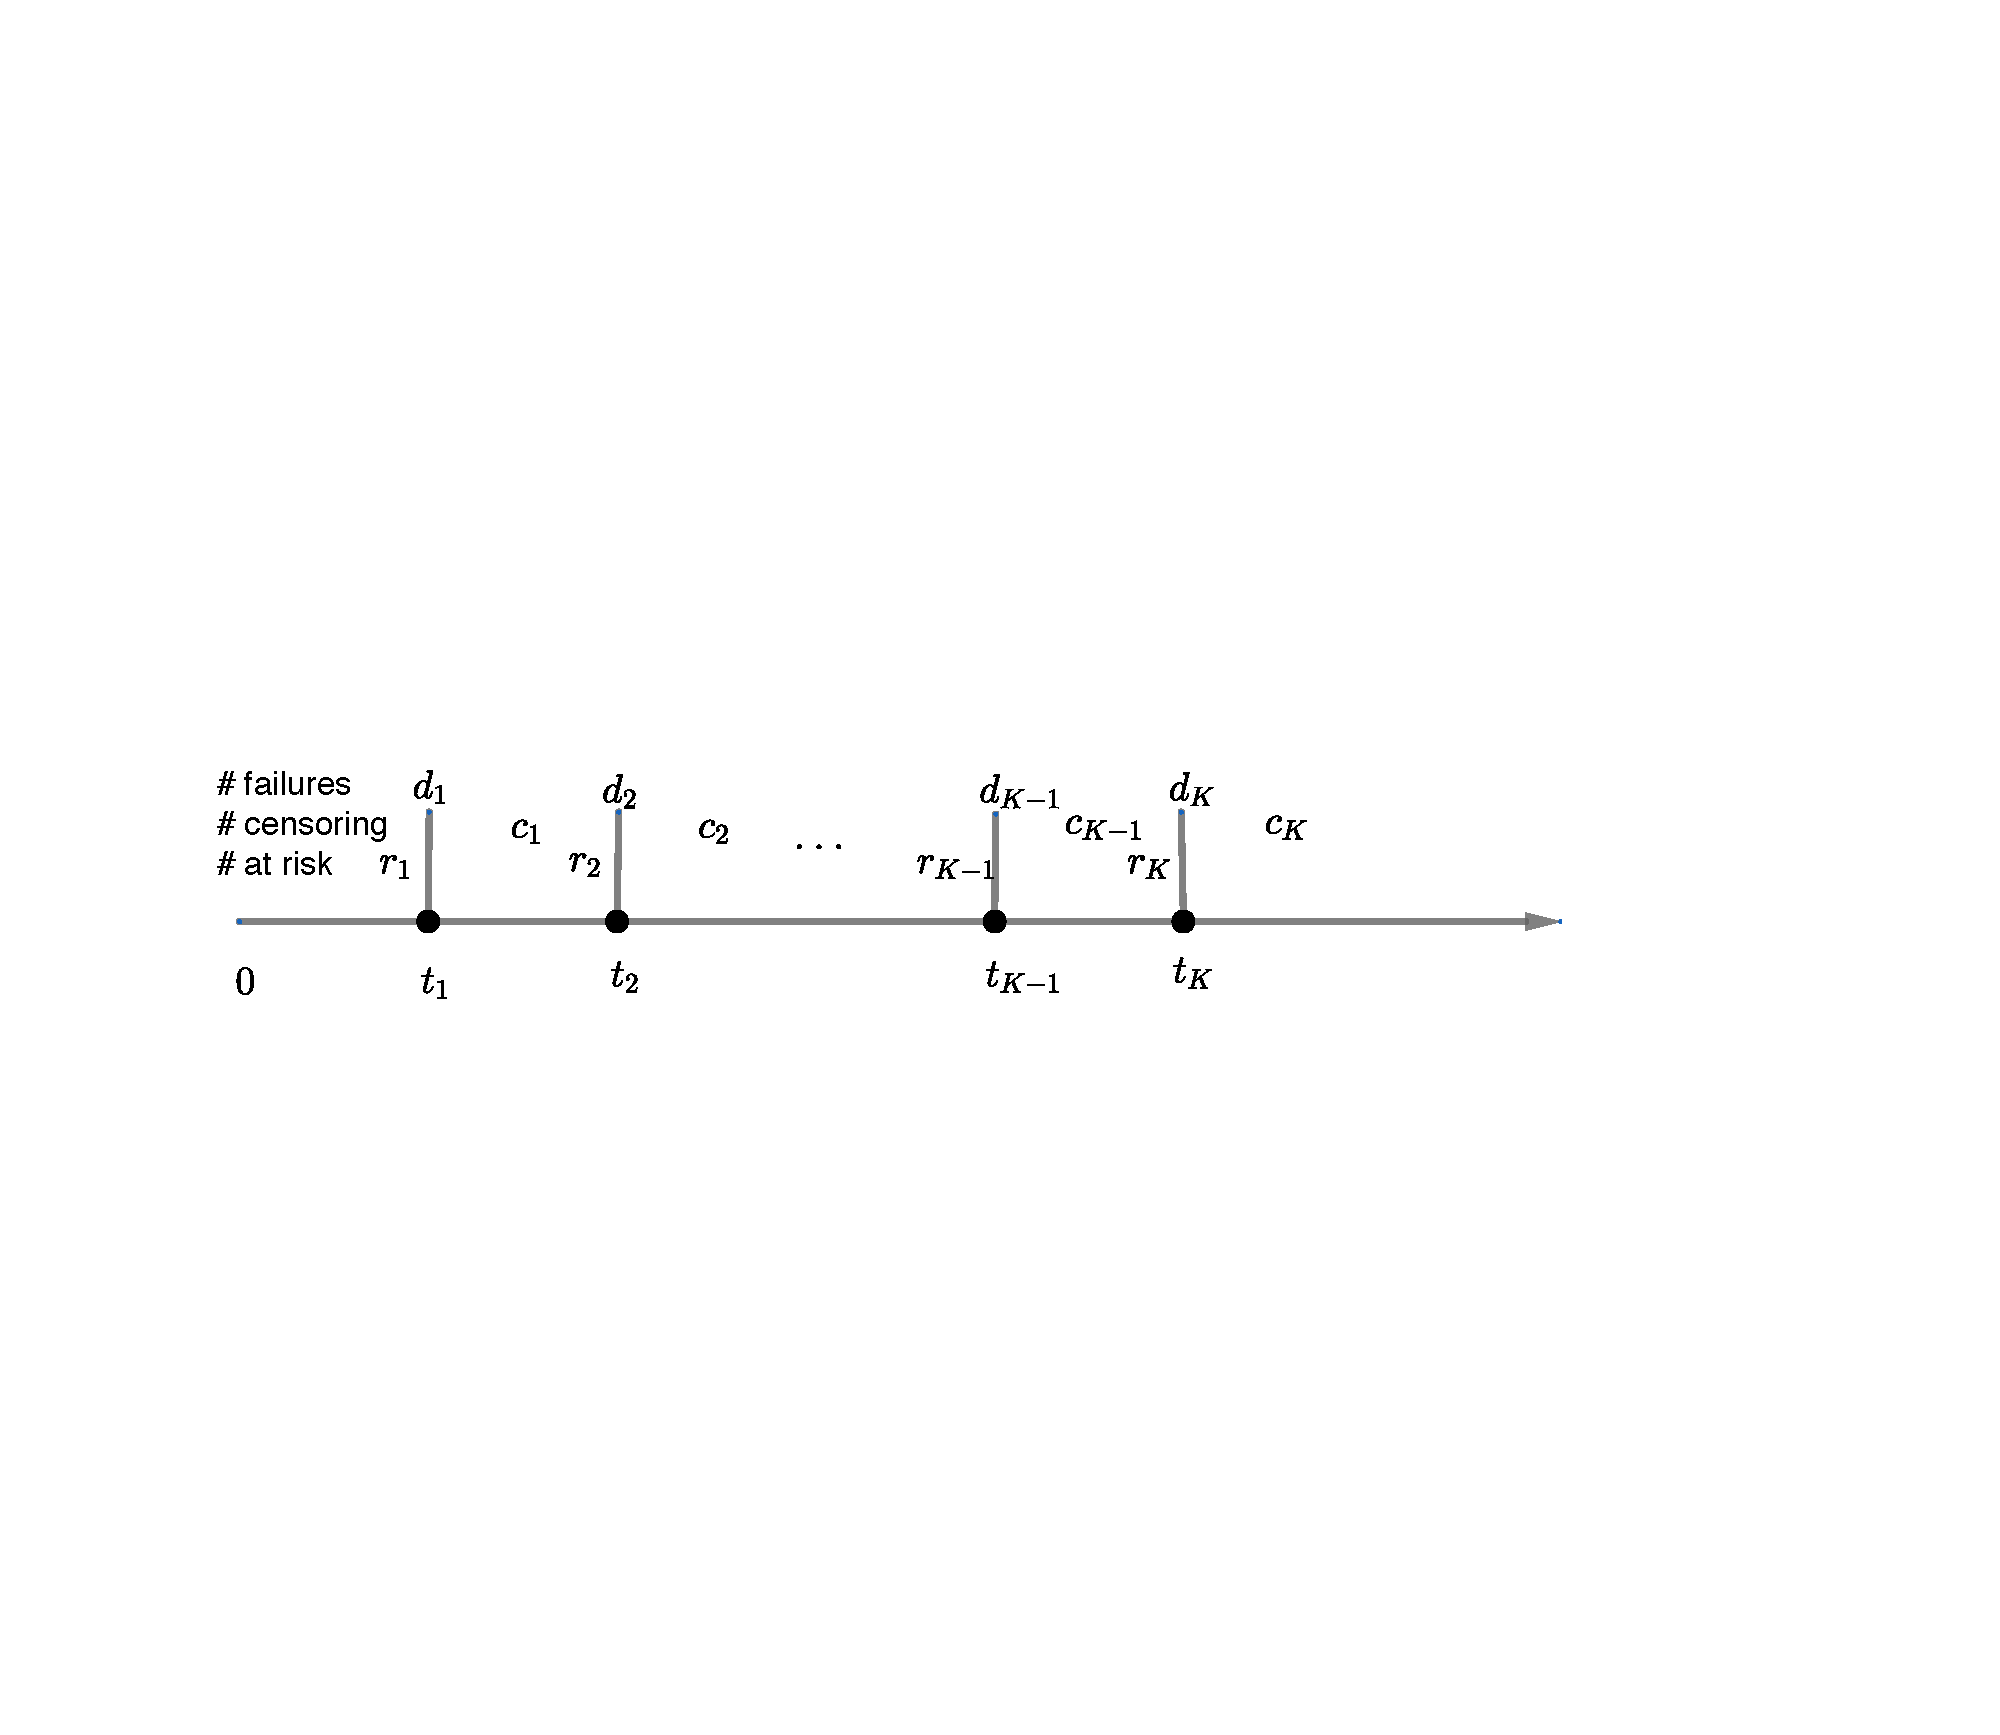
\includegraphics[width = \textwidth]{figures/kmcurvedata}
\caption{Data structure for the Kaplan--Meier curve}\label{fig::kmcurve-data}
\end{figure}

Figure \ref{fig::kmcurve-data} shows the common data structure with censoring in survival analysis:
\begin{enumerate}
[(S1)]
\item
$t_1,\ldots, t_K$ are the death times, and $d_1,\ldots, d_K$ are the corresponding number of deaths;

\item
$r_1, \ldots, r_K$ are the number of patients at risk, that is, $r_1$ patients are not dead or censored right before time $t_1$, and so on;

\item
$c_1,\ldots, c_K$ are the number of censored patients within interval $[t_1, t_2 ) ,\ldots, [d_K, \infty)$.
\end{enumerate}


\citet{kaplan1958nonparametric} proposed the following simple estimator for the survival function.

\begin{definition}
[Kaplan--Meier curve]\label{def::km-curve}
First estimate the discrete hazard function at the failure times $\left\{ t_{1},\ldots,t_{K}\right\} $
as $\hat{\lambda}_{k}=d_{k}/r_{k}\ (k=1,\ldots,K)$ and then estimate the survival
function as
\[
\hat{S}(t)=\prod_{k:t_{k}\leq t}(1-\hat{\lambda}_{k}).
\]
\end{definition}


The $\hat{S}(t)$ in Definition \ref{def::km-curve}  is also called the product-limit estimator
of the survival function due to its mathematical form.



At each failure time $t_{k}$, we view $d_{k}$ as the result of $r_{k}$
Bernoulli trials with probability $\lambda_{k}$. So $\hat{\lambda}_{k}=d_{k}/r_{k}$
has variance $\lambda_{k}(1-\lambda_{k})/r_{k}$ which can be estimated
by 
\[
\hat{\var}(\hat{\lambda}_{k})=\hat{\lambda}_{k}(1-\hat{\lambda}_{k})/r_{k}.
\]
We can estimate the variance of the survival function using the delta
method. We can approximate the variance of
\begin{eqnarray*}
\log\hat{S}(t) 
&=& \sum_{k:t_{k}\leq t}\log(1-\hat{\lambda}_{k}) \\ 
&\cong & \sum_{k:t_{k}\leq t}\log(1-\lambda_{k})-\sum_{k:t_{k}\leq t}(1-\lambda_{k})^{-1}(\hat{\lambda}_{k}-\lambda_{k})
\end{eqnarray*}
by
\begin{eqnarray*}
\hat{\var}\left\{ \log\hat{S}(t)\right\}  &=&\sum_{k:t_{k}\leq t}(1-\lambda_{k})^{-2}\hat{\var}(\hat{\lambda}_{k}) \\
&=&\sum_{k:t_{k}\leq t}(1-\hat{\lambda}_{k})^{-2}\hat{\lambda}_{k}(1-\hat{\lambda}_{k})/r_{k}\\
&=&\sum_{k:t_{k}\leq t}\frac{d_{k}}{r_{k}(r_{k}-d_{k})},
\end{eqnarray*}
which is called Greenwood's formula \citep{greenwood1926report}. A hidden assumption above is the independence of the $\hat{\lambda}_k$'s. This assumption cannot be justified due to the dependence of the events. However, a deeper theory of counting processes shows that  Greenwood's formula is valid even without the independence \citep{fleming2011counting}. 


Based on Greenwood's formula, we can construct a confidence interval for $\log S(t)$:
\[
\log\hat{S}(t)\pm z_{\alpha}\sqrt{\hat{\var}\left\{ \log\hat{S}(t)\right\} },
\]
which implies a confidence interval for $S(t)$. However, this interval
can be outside of range $[0,1]$ because the log transformation $\log S(t)$ is in the range of $(-\infty, 0)$ but the Normal approximation is in the range $(-\infty, \infty).$ 
A better transformation is log-log:
\[
v(t)=\log\left\{ -\log S(t)\right\} ,\quad\hat{v}(t)=\log\left\{ -\log\hat{S}(t)\right\} .
\]
Using Taylor expansion, we can approximate the variance of 
\[
\hat{v}(t)\cong\log\left\{ -\log S(t)\right\} -\frac{1}{\log S(t)}\left\{  \log \hat{S}(t)- \log S(t)\right\} 
\]
by 
\[
\frac{\hat{\var}\left\{ \log\hat{S}(t)\right\} }{\left\{ \log\hat{S}(t)\right\} ^{2}}.
\]
Based on this formula and Greenwood's formula above, we can construct
a confidence interval for $v(t)$:
\[
\log\left\{ -\log\hat{S}(t)\right\} \pm z_{\alpha}\sqrt{\hat{\var}\left\{ \log\hat{S}(t)\right\} }/\log\hat{S}(t),
\]
which implies another confidence interval for $S(t)$. 
In the \ri{R} package \ri{survival}, the function \ri{survfit} can fit the Kaplan--Meier curve, where the specifications \ri{conf.type = "log"} and \ri{conf.type = "log-log"} return confidence intervals based on the log and log-log transformations, respectively.  




Figure \ref{fig::kmcurve2x2-lin} plots four curves based on the combination of \ri{NALTREXONE} and  \ri{THERAPY} using the data of \citet{lin2016simultaneous}. I do not show the confidence intervals due to the large overlap. 

\begin{lstlisting}
> km4groups = survfit(Surv(futime, relapse) ~ NALTREXONE + THERAPY,
+                     data = COMBINE)
> plot(km4groups, bty = "n", col = 1:4,
+      xlab = "t", ylab = "survival functions")
> legend("topright",
+        c("NALTREXONE=0, THERAPY=0", 
+          "NALTREXONE=0, THERAPY=1", 
+          "NALTREXONE=1, THERAPY=0", 
+          "NALTREXONE=1, THERAPY=1"),
+        col = 1:4, lty = 1, bty = "n")
\end{lstlisting}



\begin{figure}[th]
\centering
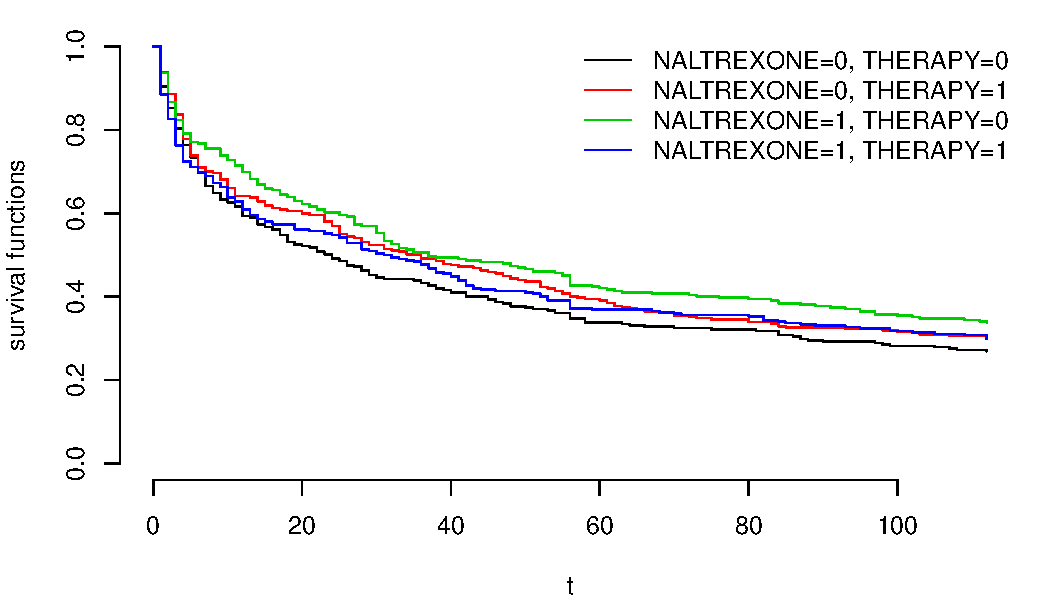
\includegraphics[width = \textwidth]{figures/KMcurve2x2.pdf}
\caption{\citet{lin2016simultaneous}'s data}\label{fig::kmcurve2x2-lin}
\end{figure}




The above discussion on the Kaplan--Meier curve is rather heuristic. More fundamentally, what is the underlying censoring mechanism that ensures the possibility that the distribution of the survival time can be recovered by the observed data? It turns out that we have implicitly assumed that the survival time and the censoring time are independent. Homework problem \ref{hw23::identification-km} gives a theoretical statement. 



\section{Cox model for time-to-event outcome}



Another important problem is to model the dependence of the survival time $T$ on covariates $x$. The major challenge is that the survival time is often censored. Let $C_i$ be the censoring time of unit $i$, and we can only observe the minimum value of the survival time and the censoring time. So the observed data are
$
(x_{i}, y_{i},\delta_{i})_{i=1}^{n}, 
$
where 
\[
y_{i}=\min(T_{i},C_{i}),\quad\delta_{i}=1(T_{i}\leq C_{i})
\]
are the event time and the censoring indicator, respectively. A key assumption is that the censoring mechanism is noninformative:
\begin{assumption}
[noninformative censoring]\label{assume::non-informative-censoring}
$
T_{i}\ind C_{i}\mid x_{i}.
$
\end{assumption}



We can start with parametric models. 

\begin{example}\label{ex::log-normal-regression}
Assume $T_i \mid x_i \sim $ Log-Normal$(x_i^{\T}\beta, \sigma^2)$. Equivalently,
$$
\log T_i = x_i^{\T}\beta + \varepsilon_i , 
$$
where the $\varepsilon_i$'s are IID $\N(0,\sigma^2)$ independent of the $x_i$'s. This is a Normal linear model on $\log T_i$. 
\end{example}
 
 
 \begin{example}\label{ex::weibull-regression}
 Assume that $T_i \mid x_i \sim$ Weibull$(a, b= e^{x_i^{\T}\beta})$. Based on the definition of the Weibull distribution in Example \ref{eq::weibull-representation}, we have
 $$
 \log T_i = x_i^{\T} \beta+ \varepsilon_i
 $$
 where the $\varepsilon_i$'s are IID $a^{-1} \log \text{Exponential}(1)$, independent of the $x_i$'s. 
 \end{example}

 
The \ri{R} package \ri{survival} contains the function \ri{survreg} to fit parametric survival models including the choices of \ri{dist = "lognormal"}, \ri{dist = "weibull"}, etc. However, these parametric models are not commonly used in practice. The parametric forms can be too strong, and due to right censoring, the inference can be driven by extrapolation to the right tail. 


\subsection{Cox model and its interpretation}

 

\citet{cox1972regression} proposed to model the conditional hazard function
\begin{eqnarray*}
\lambda(t\mid x) 
&=& \lim_{\Delta t\downarrow0}\pr(t\leq T<t+\Delta t\mid T\geq t,x)/\Delta t \\
&=&\frac{f(t\mid x)}{S(t\mid x)} .
\end{eqnarray*}
His celebrated proportional hazards model has the following form.

\begin{assumption}
[Cox proportional hazards model]\label{assume::cox-ph-model}
Assume the conditional hazard ratio function has the form
\begin{eqnarray}\label{eq::proportional-hazards-model}
\lambda(t\mid x)=\lambda_{0}(t)\exp(x^{\T}\beta) ,
\end{eqnarray}
where $\beta$ is an unknown parameter and $\lambda_{0}(\cdot)$ is an unknown function. 
\end{assumption}

Assumption \ref{assume::cox-ph-model} is equivalent to
$$
\log \lambda(t\mid x) = \log \lambda_{0}(t) + x^{\T}\beta .
$$
Unlike other regression models, $x$ does not contain the intercept in \eqref{eq::proportional-hazards-model}. If the first component of $x$ is $1$, then we can write 
\begin{eqnarray*}
\lambda(t\mid x) 
&=&\lambda_{0}(t)  \exp(x_1\beta_1 + \cdots + x_p \beta_p) \\
&=& \lambda_{0}(t) e^{\beta_1}  \exp(x_2\beta_2 + \cdots + x_p \beta_p)
\end{eqnarray*}
and redefine $\lambda_{0}(t) e^{\beta_1}$ as another unknown function. With an intercept, we cannot identify $\lambda_{0}(t) $ and $\beta_1$ separately.  So we drop the intercept to ensure identifiability. 

From the log-linear form of the conditional hazard function, we have
$$
\log \frac{\lambda(t\mid x')}{ \lambda(t\mid x)} = (x' - x)^{\T} \beta,
$$
so each coordinate of $\beta$ measures the log conditional hazard ratio holding other covariates constant. 
Because of this, \eqref{eq::proportional-hazards-model} is called the proportional hazards model. 
A positive $\beta_j$ suggests a ``positive'' effect on the hazard function and thus a ``negative'' effect on the survival time itself. 
Consider a special case with a binary $x_i$, then the proportional hazards assumption implies that $\lambda(t\mid 1) = \gamma  \lambda(t\mid 0)$ with $\gamma=\exp(\beta)$, and therefore the survival functions satisfy
\begin{eqnarray*}
S(t\mid 1) 
&=& \exp\left\{  - \int_0^t  \lambda(u\mid 1) \d u  \right\} \\
&=&  \exp\left\{  - \gamma  \int_0^t  \lambda(u\mid 0) \d u  \right\}  \\
&=& \left\{  S(t\mid 0) \right\}^\gamma,
\end{eqnarray*}
which is a power transformation. 
Qualitatively, we have the following two cases:
\begin{enumerate}
[(PH1)]
\item
$\beta <0$: so the hazard ratio $\gamma = \exp(\beta) < 1$ and $S(t\mid 1) \geq  S(t\mid 0)$ for all $t$, which implies a longer survival time under treatment;
\item 
$\beta >0$: so the hazard ratio $\gamma = \exp(\beta) > 1$ and $S(t\mid 1) \leq  S(t\mid 0)$ for all $t$, which implies a shorter survival time under treatment.
\end{enumerate}
Figure \ref{fig::ph-assumptions} shows some survival functions satisfying the proportional hazards assumption, none of which cross each other within the interval $t\in (0,\infty).$ When the two survival functions cross, the proportional hazards assumption does not hold. 


\begin{figure}
\centering
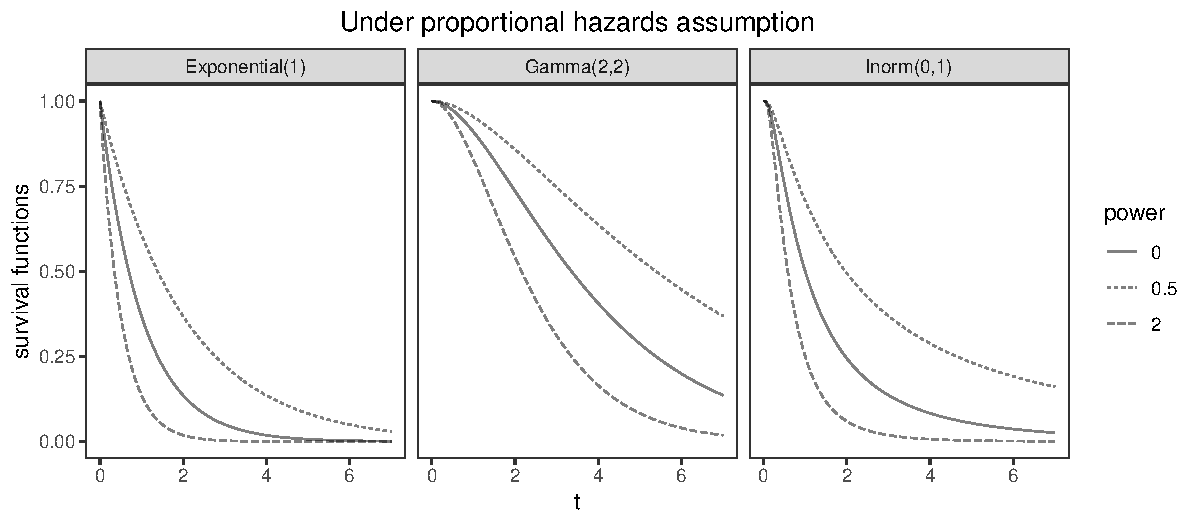
\includegraphics[width = \textwidth]{figures/ph_survival_curves.pdf}
\caption{Proportional hazards assumption with different baseline survival functions, where the power equals $\gamma = \exp(\beta)$.
}\label{fig::ph-assumptions}
\end{figure}

Theoretically, we can allow the covariates to be time-dependent, that is, $x_i(t)$ can depend on $t$ and thus is a stochastic process. However, the interpretation of the coefficient becomes challenging \citep{fisher1999time}. This chapter focuses on the simple case with time-invariant covariates. 




\subsection{Partial likelihood}


The likelihood function is rather complicated, which depends on an unknown function $\lambda_0(t)$. 
Assuming no ties, \citet{cox1972regression} proposed to use the partial likelihood function
to estimate $\beta$:
\[
L(\beta)=\prod_{k=1}^{K}\frac{\exp(x_{k}^{\T}\beta)}{\sum_{l\in R(t_{k})}\exp(x_{l}^{\T}\beta)},
\]
where the product is over $K$ time points with failures, $x_k$ is the covariate value of the failure at time $t_k$, and $R(t_k)$ contains the indices of the units at risk at time $t_k$, i.e., the units not censored or failed right before the time $t_k$. 


\citet{freedman2008survival} gives a heuristic explanation of the partial likelihood based on the following results which extends Proposition \ref{prop::minimum-expo} on the Exponential distribution. 

\begin{theorem}
\label{thm::freedman-explain-cox}
If $T_1,\ldots, T_n$ are independent with hazard function $\lambda_i(t)$ $(i=1,\ldots, n)$, then their minimum value $\underline{T} = \min_{1\leq i \leq n} T_i$ has hazard function $\sumn \lambda_i(t)$.
Moreover, if $\lambda_i(t) = c_i \lambda(t)$, then 
$$
\pr (  T_i = \underline{T}  ) = \frac{c_i}{ \sum_{i'=1}^n  c_{i'} }.
$$
\end{theorem} 

\begin{myproof}{Theorem}{\ref{thm::freedman-explain-cox}}
The survival function of $\underline{T} $ is
\begin{eqnarray*}
\pr (  \underline{T} > t  ) 
&=& \pr(  T_1>t,\ldots, T_n>t ) \\
&=& \prod_{i=1}^n S_i(t) ,
\end{eqnarray*}
so Proposition \ref{prop::hazard-pdf-survival} implies that its hazard function is
\begin{eqnarray*}
- \frac{\d}{\d t} \log \pr ( \underline{T} > t )  
&=& \sumn \left\{ - \frac{\d}{\d t} \log   S_i(t) \right\} \\
&=& \sumn \lambda_i(t). 
\end{eqnarray*}
So the first conclusion follows. 
 
 
As a byproduct of the above proof, the density of $\underline{T} $ is $\sumn \lambda_i(t) \prod_{i=1}^n S_i(t)$ based in Proposition \ref{prop::hazard-pdf-survival}. It must have integral one; with $\lambda_i(t) = c_i \lambda(t)$, this implies 
\begin{equation}
\left( \sumn c_i  \right) \int_0^{\infty} \lambda(t) \prod_{i=1}^n S_i(t) \d t = 1.
\label{eq::integral1-minimum-Ts}
\end{equation}
Therefore, we have 
\begin{eqnarray*}
\pr ( T_i = \underline{T}   ) 
&=& \pr\{ T_i \leq T_{i'} \text{ for all } i' \neq i  \} \\
&=& \int_0^{\infty}   \prod_{i' \neq i} S_{i'}(t)  f_i(t) \d t\\
&=&  \int_0^{\infty}   \prod_{i'=1}^n S_{i'}(t)  \lambda_i(t) \d t \\
&=& c_i  \int_0^{\infty}  \lambda(t)   \prod_{i'=1}^n S_{i'}(t)  \d t \\
&=& c_i  \Big /  \sumn c_{i'},
\end{eqnarray*}
where the last equality holds due to \eqref{eq::integral1-minimum-Ts}. 
\end{myproof}

Theorem \ref{thm::freedman-explain-cox} explains each of the $K$ components in the partial likelihood. At time $t_k$, the units in $R(t_k)$ are all at risk, and unit $k$ fails, assuming no ties. The probability that unit $k$ has the smallest failure time among units in $R(t_k)$ is 
$$
 \frac{   \exp(x_k^{\T} \beta)  }{ \sum_{l\in R(t_k)}    \exp(x_l^{\T} \beta) } 
$$
from Theorem \ref{thm::freedman-explain-cox}. The product in the partial likelihood is based on the independence of the events at the $K$ failure times, which is more difficult to justify. A rigorous justification relies on the deeper theory of counting processes \citep{fleming2011counting} or semiparametric statistics \citep{tsiatis2007semiparametric}. 



The log-likelihood function is
\[
\log L(\beta)=\sum_{k=1}^{K}\left\{ x_{k}^{\T}\beta-\log\sum_{l\in R(t_{k})}\exp(x_{l}^{\T}\beta)\right\} ,
\]
and the score function is
\[
\frac{\partial\log L(\beta)}{\partial\beta}=\sum_{k=1}^{K}\left\{ x_{k}-\frac{\sum_{l\in R(t_{k})}\exp(x_{l}^{\T}\beta)x_{l}}{\sum_{l\in R(t_{k})}\exp(x_{l}^{\T}\beta)}\right\} .
\]
Define 
\[
\pi_{\beta}(l\mid R_{k})=\exp(x_{l}^{\T}\beta)/\sum_{l\in R(t_{k})}\exp(x_{l}^{\T}\beta),\quad(l\in R(t_{k}))
\]
which sum to one, so they induce a probability measure leading to
expectation $E_{\beta}(\cdot\mid R_{k})$ and covariance $\cov_{\beta}(\cdot\mid R_{k})$.
With this notation, the score function simplifies to
\[
\frac{\partial\log L(\beta)}{\partial\beta}=\sum_{k=1}^{K}\left\{ x_{k}-E_{\beta}(x\mid R_{k})\right\} ,
\]
where 
$
E_{\beta}(x\mid R_{k}) = \sum_{l\in R(t_{k})}  \pi_{l}(\beta\mid R_{k}) x_l;
$
the Hessian matrix simplifies to
$$
\frac{\partial^{2}\log L(\beta)}{\partial\beta\partial\beta^{\T}}  =-\sum_{k=1}^{K}\cov_{\beta}(x\mid R_{k})\preceq 0,
$$
where
\begin{eqnarray*}
&&\cov_{\beta}(x\mid R_{k}) \\
&=&  \begin{pmatrix}
\sum_{l\in R(t_{k})}\exp(x_{l}^{\T}\beta)x_{l}x_{l}^{\T}\sum_{l\in R(t_{k})}\exp(x_{l}^{\T}\beta) \\
-\sum_{l\in R(t_{k})}\exp(x_{l}^{\T}\beta)x_{l}\sum_{l\in R(t_{k})}\exp(x_{l}^{\T}\beta)x_{l}^{\T} 
\end{pmatrix}   \Big / \left\{ \sum_{l\in R(t_{k})}\exp(x_{l}^{\T}\beta)\right\} ^{2} \\
&=&
\sum_{l\in R(t_{k})}\pi_{\beta}(l\mid R_{k})x_{l}x_{l}^{\T}-\sum_{l\in R(t_{k})}\pi_{\beta}(l\mid R_{k})x_{l}\sum_{l\in R(t_{k})}\pi_{\beta}(l\mid R_{k})x_{l}^{\T} . 
\end{eqnarray*}
%
%
% $\cov_{\beta}(x\mid R_{k}) $ equals 
%\begin{eqnarray*}
%\frac{\sum_{l\in R(t_{k})}\exp(x_{l}^{\T}\beta)x_{l}x_{l}^{\T}\sum_{l\in R(t_{k})}\exp(x_{l}^{\T}\beta)-\sum_{l\in R(t_{k})}\exp(x_{l}^{\T}\beta)x_{l}\sum_{l\in R(t_{k})}\exp(x_{l}^{\T}\beta)x_{l}^{\T}}{\left\{ \sum_{l\in R(t_{k})}\exp(x_{l}^{\T}\beta)\right\} ^{2}}\\
%=
%\sum_{l\in R(t_{k})}\pi_{\beta}(l\mid R_{k})x_{l}x_{l}^{\T}-\sum_{l\in R(t_{k})}\pi_{\beta}(l\mid R_{k})x_{l}\sum_{l\in R(t_{k})}\pi_{\beta}(l\mid R_{k})x_{l}^{\T} . 
%\end{eqnarray*}
 

The \ri{coxph} function in the \ri{R} package \ri{survival} uses Newton's method to compute the maximizer $\hat{\beta}$ of the partial likelihood function, and uses the inverse of the observed Fisher information to approximate its asymptotic variance. 
\citet{lin1989robust} proposed a sandwich covariance estimator to allow for the misspecification of the Cox model.  The \ri{coxph} function with \ri{robust = TRUE} reports the corresponding robust standard errors. 



\subsection{Examples}
Using \citet{lin2016simultaneous}'s data, we have the following results. 

\begin{lstlisting}
> cox.fit <- coxph(Surv(futime, relapse) ~ NALTREXONE*THERAPY + 
+                    AGE + GENDER + T0_PDA + site,
+                  data=COMBINE)
> summary(cox.fit)
Call:
coxph(formula = Surv(futime, relapse) ~ NALTREXONE * THERAPY + 
    AGE + GENDER + T0_PDA + site, data = COMBINE)

  n= 1226, number of events= 856 

                        coef exp(coef)  se(coef)      z Pr(>|z|)    
NALTREXONE         -0.249719  0.779020  0.097690 -2.556  0.01058 *  
THERAPY            -0.167050  0.846158  0.096102 -1.738  0.08217 .  
AGE                -0.015540  0.984580  0.003559 -4.366 1.27e-05 ***
GENDERmale         -0.140621  0.868818  0.075368 -1.866  0.06207 .  
T0_PDA              0.002550  1.002553  0.001368  1.863  0.06242 .  
sitesite_1         -0.091853  0.912239  0.167261 -0.549  0.58290    
sitesite_10        -0.227185  0.796774  0.175427 -1.295  0.19531    
sitesite_2          0.121236  1.128892  0.160052  0.757  0.44876    
sitesite_3         -0.084483  0.918987  0.161121 -0.524  0.60004    
sitesite_4         -0.471612  0.623996  0.175203 -2.692  0.00711 ** 
sitesite_5         -0.128286  0.879602  0.161782 -0.793  0.42780    
sitesite_6         -0.240563  0.786185  0.161958 -1.485  0.13745    
sitesite_7          0.372004  1.450639  0.157616  2.360  0.01827 *  
sitesite_8          0.067700  1.070045  0.160876  0.421  0.67388    
sitesite_9          0.267373  1.306528  0.154911  1.726  0.08435 .  
NALTREXONE:THERAPY  0.337539  1.401495  0.137441  2.456  0.01405 *  
\end{lstlisting}

\ri{NALTREXONE} has a significant negative log hazard ratio, but \ri{THERAPY} has a nonsignificant negative log hazard ratio. More interestingly, their interaction \ri{NALTREXONE:THERAPY} has a significant positive log hazard ratio. This suggests that combining \ri{NALTREXONE} and \ri{THERAPY} is worse than using \ri{NALTREXONE} alone to delay the first time of heavy drinking and other endpoints. This is also coherent with the survival curves in Figure \ref{fig::kmcurve2x2-lin}, in which the best Kaplan--Meier curve corresponds to \ri{NALTREXONE=1, THERAPY=0}.





Using \citet{keele2010proportionally}'s data, we have the following results:

\begin{lstlisting}
> cox.fit <- coxph(Surv(acttime, censor) ~ 
+                    hcomm + hfloor + scomm + sfloor + 
+                    prespart + demhsmaj + demsnmaj + 
+                    prevgenx + lethal + 
+                    deathrt1 + acutediz + hosp01  + 
+                    hospdisc  + hhosleng + 
+                    mandiz01 + femdiz01 + peddiz01 + orphdum + 
+                    natreg + I(natreg^2) + vandavg3 + wpnoavg3 + 
+                    condavg3 + orderent + stafcder, 
+                data=fda)
> summary(cox.fit)
Call:
coxph(formula = Surv(acttime, censor) ~ hcomm + hfloor + scomm + 
    sfloor + prespart + demhsmaj + demsnmaj + prevgenx + lethal + 
    deathrt1 + acutediz + hosp01 + hospdisc + hhosleng + mandiz01 + 
    femdiz01 + peddiz01 + orphdum + natreg + I(natreg^2) + vandavg3 + 
    wpnoavg3 + condavg3 + orderent + stafcder, data = fda)

  n= 408, number of events= 262 

                  coef  exp(coef)   se(coef)      z Pr(>|z|)    
hcomm        3.642e-01  1.439e+00  2.951e+00  0.123 0.901775    
hfloor       7.944e+00  2.819e+03  8.173e+00  0.972 0.331071    
scomm        4.716e-01  1.603e+00  1.898e+00  0.248 0.803771    
sfloor       2.604e+00  1.352e+01  2.370e+00  1.099 0.271877    
prespart     8.038e-01  2.234e+00  3.042e-01  2.643 0.008226 ** 
demhsmaj     1.363e+00  3.909e+00  1.917e+00  0.711 0.476890    
demsnmaj     1.217e+00  3.377e+00  5.606e-01  2.171 0.029940 *  
prevgenx    -9.915e-04  9.990e-01  7.779e-04 -1.275 0.202459    
lethal       7.872e-02  1.082e+00  2.378e-01  0.331 0.740605    
deathrt1     6.537e-01  1.923e+00  2.435e-01  2.685 0.007253 ** 
acutediz     1.994e-01  1.221e+00  2.262e-01  0.882 0.377896    
hosp01       4.280e-02  1.044e+00  2.495e-01  0.172 0.863768    
hospdisc    -1.238e-06  1.000e+00  5.278e-07 -2.345 0.019002 *  
hhosleng    -1.273e-02  9.874e-01  1.988e-02 -0.640 0.521891    
mandiz01    -1.177e-01  8.889e-01  3.800e-01 -0.310 0.756711    
femdiz01     9.032e-01  2.468e+00  3.497e-01  2.583 0.009799 ** 
peddiz01    -3.401e-02  9.666e-01  5.112e-01 -0.067 0.946968    
orphdum      5.540e-01  1.740e+00  2.109e-01  2.626 0.008630 ** 
natreg      -2.221e-02  9.780e-01  8.282e-03 -2.682 0.007318 ** 
I(natreg^2)  1.029e-04  1.000e+00  4.567e-05  2.253 0.024276 *  
vandavg3    -2.014e-02  9.801e-01  1.536e-02 -1.311 0.189802    
wpnoavg3     5.220e-03  1.005e+00  1.426e-03  3.660 0.000252 ***
condavg3     9.628e-03  1.010e+00  2.271e-02  0.424 0.671637    
orderent    -1.810e-02  9.821e-01  8.147e-03 -2.222 0.026296 *  
stafcder     8.013e-04  1.001e+00  7.986e-04  1.003 0.315719    
\end{lstlisting}





\subsection{Log-rank test as a score test from Cox model}


A standard problem in clinical trials is to compare the survival times under treatment and control. Assume no ties in the failure times, and let $x$ denote the binary indicator for treatment. 
Under the proportional hazards assumption, the
control group has hazard $\lambda_{0}(t)$, and the treatment group has
hazard $\lambda_{1}(t) = \lambda_{0}(t)e^{\beta}.$ We are interested in testing the null hypothesis 
$$
\beta=0 \Longleftrightarrow \lambda_{1}(t) = \lambda_{0}(t) \Longleftrightarrow S_{1}(t) = S_{0}(t).
$$


Under the null hypothesis, the
score function reduces to
\begin{eqnarray*}
\frac{\partial\log L(\beta)}{\partial\beta}\Big|_{\beta=0} 
&=&\sum_{k=1}^{K}\left\{ x_{k}-E_{\beta=0}(x\mid R_{k})\right\} \\
&=&\sum_{k=1}^{K}\left(x_{k}-\frac{r_{k1}}{r_{k}}\right),
\end{eqnarray*}
because 
\[
E_{\beta=0}(x\mid R_{k})=\frac{\sum_{l\in R(t_{k})}x_{l}}{\sum_{l\in R(t_{k})}1}=\frac{r_{k1}}{r_{k}}
\]
equaling the ratio of the number of treated units at risk $r_{k1}$ over the
number of units at risk $r_k$, at time $t_k$. The Fisher information at the null is
\begin{eqnarray*}
-\frac{\partial^{2}\log L( 0 )}{\partial\beta\partial\beta^{\T}} 
&=& \sum_{k=1}^{K}\cov_{\beta=0}(x\mid R_{k}) \\
&=& \sum_{k=1}^{K}\frac{r_{k1}}{r_{k}}\left(1-\frac{r_{k1}}{r_{k}}\right).
\end{eqnarray*}

The score test for classical parametric models relies on  
$$
\frac{\partial\log L( 0 )}{\partial\beta}  \asim \N \left(0,  -\frac{\partial^{2}\log L( 0 )}{\partial\beta\partial\beta^{\T}}   \right),
$$
which follows from Bartlett's identity and the CLT. Applying this fact to Cox's model, we have
\[
\text{LR} = \frac{\sum_{k=1}^{K}\left(x_{k}-\frac{r_{k1}}{r_{k}}\right)}{\sqrt{\sum_{k=1}^{K}\frac{r_{k1}}{r_{k}}\left(1-\frac{r_{k1}}{r_{k}}\right)}}\asim\N(0,1).
\]
So we reject the null at level $\alpha$ if $|\text{LR} | $ is larger than the upper $1-\alpha/2$ quantile of standard Normal. This
is almost identical to the log-rank test without ties. Allowing for ties, \citet{mantel1966evaluation} proposed a more general form of the log-rank test\footnote{\citet{peto1972asymptotically} popularized the name log-rank test.}.


The \ri{survdiff} function in the \ri{survival} package implements various tests including the log-rank test as a special case. Below, I use the \ri{gehan} dataset in the \ri{MASS} package to illustrate the log rank test. The data were from a matched-pair experiment of 42 leukaemia patients \citep{gehan1965generalized}. Treated units received the drug 6-mercaptopurine, and the rest are controls. For illustration purposes, I ignore the pair indicators. 


 

\begin{lstlisting}
> library(MASS)
> head(gehan)
  pair time cens   treat
1    1    1    1 control
2    1   10    1    6-MP
3    2   22    1 control
4    2    7    1    6-MP
5    3    3    1 control
6    3   32    0    6-MP
> survdiff(Surv(time, cens) ~ treat,
+          data = gehan)
Call:
survdiff(formula = Surv(time, cens) ~ treat, data = gehan)

               N Observed Expected (O-E)^2/E (O-E)^2/V
treat=6-MP    21        9     19.3      5.46      16.8
treat=control 21       21     10.7      9.77      16.8

 Chisq= 16.8  on 1 degrees of freedom, p= 4e-05 
 \end{lstlisting}
 
 

The treatment was quite effective, yielding an extremely small $p$-value even with moderate sample size. It is also clear from the Kaplan--Meier curves in Figure \ref{fig:: gehan_kmcurve-data} and the results from fitting the Cox proportional hazards model. 

\begin{figure}[th]
\centering
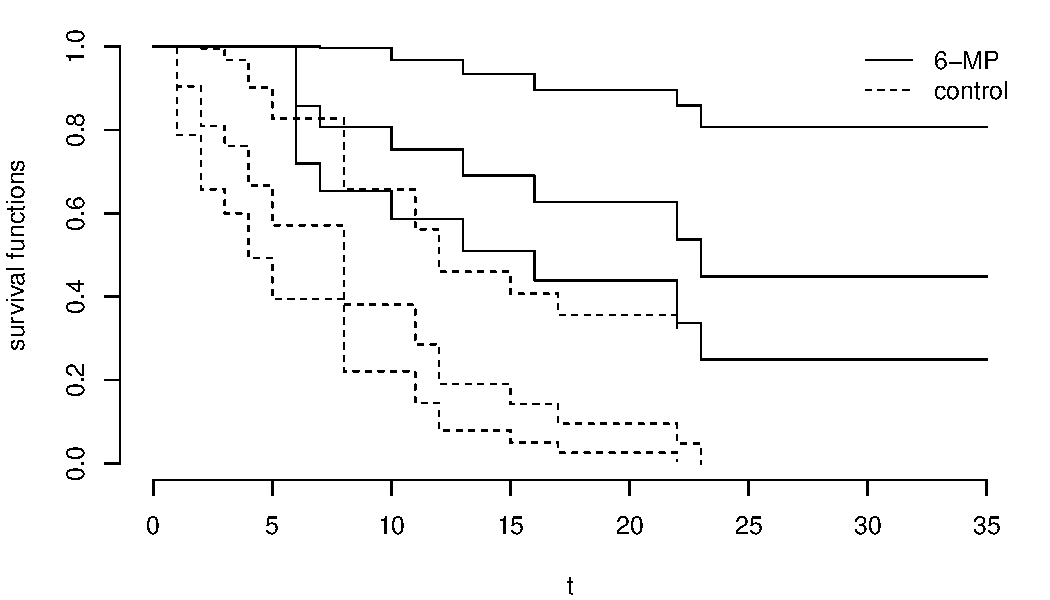
\includegraphics[width = \textwidth]{figures/gehan_kmcurve}
\caption{Kaplan--Meier curves with 95\% confidence intervals based on \citet{gehan1965generalized}'s data}\label{fig:: gehan_kmcurve-data}
\end{figure}


\begin{lstlisting}
> cox.gehan = coxph(Surv(time, cens) ~ treat,
+                     data = gehan)
> summary(cox.gehan)
Call:
coxph(formula = Surv(time, cens) ~ treat, data = gehan)

  n= 42, number of events= 30 

               coef exp(coef) se(coef)     z Pr(>|z|)    
treatcontrol 1.5721    4.8169   0.4124 3.812 0.000138 ***

             exp(coef) exp(-coef) lower .95 upper .95
treatcontrol     4.817     0.2076     2.147     10.81

Concordance= 0.69  (se = 0.041 )
Likelihood ratio test= 16.35  on 1 df,   p=5e-05
Wald test            = 14.53  on 1 df,   p=1e-04
Score (logrank) test = 17.25  on 1 df,   p=3e-05
\end{lstlisting}


The log-rank test is a standard tool in survival analysis. However, what it delivers is just a special case of the Cox proportional hazards model. The $p$-value from the log-rank test is close to the $p$-value from the score test of the Cox proportional hazards model with only a binary treatment indicator. The latter can also adjust for other pretreatment covariates. 

 
 
\section{Extensions}


\subsection{Stratified Cox model}

Many randomized trials are stratified. The Combined Pharmacotherapies and Behavioral Interventions study reviewed at the beginning of this chapter is an example with \ri{site} indicating the strata. The previous analysis includes the dummy variables of  \ri{site} in the Cox model. An alternative more flexible model is to allow for different baseline hazard functions across strata. Technically, assume
$$
\lambda_s(t \mid x) = \lambda_s(t) \exp(\beta^{\T} x)
$$
for strata $s = 1,\ldots, S$, where $\beta$ is an unknown parameter and $\{ \lambda_1(\cdot), \ldots, \lambda_S(\cdot) \}$ are unknown functions. Therefore, within each stratum $s$, the proportional hazards assumption holds; across strata, the proportional hazard assumption may not hold. Within stratum $s$, we can obtain the partial likelihood $L_s(\beta)$; by independence of the data across strata, we can obtain the joint partial likelihood 
$$
\prod_{s=1}^S L_s(\beta) .
$$
Based on the standard procedure, we can obtain the MLE and conduct inference based on the large-sample theory. The \ri{coxph} function can naturally allow for stratification with the \ri{ + strata()} in the regression formula.

\begin{lstlisting}
> cox.fit <- coxph(Surv(futime, relapse) ~ NALTREXONE*THERAPY + 
+                    AGE + GENDER + T0_PDA + strata(site), 
+                  robust = TRUE, 
+                  data=COMBINE)
> summary(cox.fit)
Call:
coxph(formula = Surv(futime, relapse) ~ NALTREXONE * THERAPY + 
    AGE + GENDER + T0_PDA + strata(site), data = COMBINE, robust = TRUE)

  n= 1226, number of events= 856 

                        coef exp(coef)  se(coef) robust se      z Pr(>|z|)
NALTREXONE         -0.252239  0.777059  0.097788  0.096437 -2.616  0.00891
THERAPY            -0.173456  0.840754  0.096258  0.095958 -1.808  0.07066
AGE                -0.015104  0.985010  0.003554  0.003512 -4.301  1.7e-05
GENDERmale         -0.139837  0.869500  0.075388  0.076580 -1.826  0.06785
T0_PDA              0.002747  1.002751  0.001369  0.001350  2.035  0.04182
NALTREXONE:THERAPY  0.335671  1.398879  0.137676  0.136890  2.452  0.01420
                      
NALTREXONE         ** 
THERAPY            .  
AGE                ***
GENDERmale         .  
T0_PDA             *  
NALTREXONE:THERAPY *  

                   exp(coef) exp(-coef) lower .95 upper .95
NALTREXONE            0.7771     1.2869    0.6432    0.9387
THERAPY               0.8408     1.1894    0.6966    1.0147
AGE                   0.9850     1.0152    0.9783    0.9918
GENDERmale            0.8695     1.1501    0.7483    1.0103
T0_PDA                1.0028     0.9973    1.0001    1.0054
NALTREXONE:THERAPY    1.3989     0.7149    1.0697    1.8294

Concordance= 0.561  (se = 0.011 )
Likelihood ratio test= 35.24  on 6 df,   p=4e-06
Wald test            = 33.85  on 6 df,   p=7e-06
Score (logrank) test = 34.94  on 6 df,   p=4e-06,   Robust = 34.15  p=6e-06
\end{lstlisting} 




\subsection{Clustered Cox model}


 With clustered data, we must adjust for the standard errors. The \ri{coxph} function reports the cluster-robust standard errors with the specification of \ri{cluster}. A canonical example of clustered data is from the matched-pair design if we view the pairs as clusters. The example below uses the data from \citet{huster1989modelling} in which two eyes of a patient were either assigned to treatment or control. 
 
 \begin{lstlisting}
 > library("timereg")
> data(diabetes)
> pair.cox = coxph(Surv(time, status) ~ treat + adult + agedx,
+                  robust = TRUE, 
+                  data = diabetes)
> summary(pair.cox)
Call:
coxph(formula = Surv(time, status) ~ treat + adult + agedx, data = diabetes, 
    robust = TRUE)

  n= 394, number of events= 155 

           coef exp(coef)  se(coef) robust se      z Pr(>|z|)
treat -0.781483  0.457727  0.168977  0.170112 -4.594 4.35e-06
adult -0.136967  0.871999  0.289344  0.270909 -0.506    0.613
agedx  0.007836  1.007866  0.009681  0.009360  0.837    0.403
         
treat ***
adult    
agedx    

      exp(coef) exp(-coef) lower .95 upper .95
treat    0.4577     2.1847    0.3279    0.6389
adult    0.8720     1.1468    0.5128    1.4829
agedx    1.0079     0.9922    0.9895    1.0265

Concordance= 0.596  (se = 0.024 )
Likelihood ratio test= 23.13  on 3 df,   p=4e-05
Wald test            = 21.54  on 3 df,   p=8e-05
Score (logrank) test = 23.01  on 3 df,   p=4e-05,   Robust = 22.09  p=6e-05

  (Note: the likelihood ratio and score tests assume independence of
     observations within a cluster, the Wald and robust score tests do not).
> pair.cox = coxph(Surv(time, status) ~ treat + adult + agedx,
+                  robust = TRUE, cluster = id,
+                  data = diabetes)
> summary(pair.cox)
Call:
coxph(formula = Surv(time, status) ~ treat + adult + agedx, data = diabetes, 
    robust = TRUE, cluster = id)

  n= 394, number of events= 155 

           coef exp(coef)  se(coef) robust se      z Pr(>|z|)
treat -0.781483  0.457727  0.168977  0.148330 -5.269 1.37e-07
adult -0.136967  0.871999  0.289344  0.295239 -0.464    0.643
agedx  0.007836  1.007866  0.009681  0.010272  0.763    0.446
         
treat ***
adult    
agedx    

      exp(coef) exp(-coef) lower .95 upper .95
treat    0.4577     2.1847    0.3423    0.6122
adult    0.8720     1.1468    0.4889    1.5553
agedx    1.0079     0.9922    0.9878    1.0284

Concordance= 0.596  (se = 0.023 )
Likelihood ratio test= 23.13  on 3 df,   p=4e-05
Wald test            = 28.55  on 3 df,   p=3e-06
Score (logrank) test = 23.01  on 3 df,   p=4e-05,   Robust = 26.55  p=7e-06

  (Note: the likelihood ratio and score tests assume independence of
     observations within a cluster, the Wald and robust score tests do not).
 \end{lstlisting}    


\subsection{Penalized Cox model}


The \ri{glmnet} package implements the penalized version of the Cox model.   
 


\section{Critiques on survival analysis}


The Kaplan--Meier curve and the Cox proportional hazards model are standard tools for analyzing medical data with censored survival times. They are among the most commonly used methods in medical journals. \citet{kaplan1958nonparametric} and \citet{cox1972regression} are two of the most cited papers in statistics. 

\citet{freedman2008survival} criticized these two standard tools. Both rely on the critical assumption of noninformative censoring that censoring and survival time are independent or conditionally independent given covariates. When censoring is due to administrative constraints, this may be a plausible assumption. The data from \citet{lin2016simultaneous} is a convincing example of noninformative censoring.  However, many other studies have more complex censoring mechanisms, for example, one may drop out of the study, and another may be killed by an irrelevant cause. The Cox model relies on an additional assumption of proportional hazards. This particular functional form facilitates the interpretation of the coefficients as log conditional hazard ratios if the model is correctly specified. However, its interpretation becomes obscure when the model is mis-specified.  Two survival curves based on \citet{lin2016simultaneous} 's data cross each other, which makes the proportional hazards assumption dubious. 


\citet{hernan2010hazards} offered a more fundamental critique on hazard-based survival analysis. For example, in a randomized treatment-control experiment, the hazard ratio at time $t$ is the ratio of the instantaneous probability of death conditioning on the event that the patients have survived up to time $t$:
$$
\frac{   \lim_{\Delta t\downarrow0}\pr(t\leq T<t+\Delta t\mid x=1, T\geq t)/\Delta t  }
{  \lim_{\Delta t\downarrow0}\pr(t\leq T<t+\Delta t\mid x=0, T\geq t)/\Delta t  }
$$
This ratio is difficult to interpret because patients who have survived up to time $t$ can be quite different in treatment and control groups, especially when the treatment is effective. Even though patients are randomly assigned at the baseline, the survivors up to time $t$ are not. \citet{hernan2010hazards} suggested focusing on the comparison of the survival functions. 




\section{Homework problems}


\paragraph{Identifiability of the survival time under independent censoring}\label{hw23::identification-km}

Assume the survival time $T$ and censoring time $C$ are continuous and independent random variables. But we can only observe $y = \min(T, C)$ and $\delta = 1(T \leq C)$. Show that the hazard function of $T$ can be identified by the following formula: 
$$
\lambda_T(t) =    \frac{   \pr(y = t, \delta = 1)   }{  \pr(y \geq t)  } . 
$$ 

 
 

\paragraph{Log-Normal regression model}

Does the log-Normal regression model in Example \ref{ex::log-normal-regression} satisfy the proportional hazards assumption?
Based on
$(y_{i},x_{i},\delta_{i})_{i=1}^{n}$, what is the likelihood function under Assumption \ref{assume::non-informative-censoring}? 
Compare it with the partial likelihood function. 


\paragraph{Weibull random variable}
\label{hw23::weibull-rv}

Using \eqref{eq::weibull-representation} to show the formulas of density, survival, and hazard functions. Calculate its mean and variance. 

Hint: Use the Gamma function to express the moments.


\paragraph{Weibull regression model}
\label{hw23::weibull-regression}


Find the distribution of
$\varepsilon_i$ in the Weibull regression model in Example \ref{ex::weibull-regression}. 
Show $E(T \mid x )$ is log-linear in $x$, and $E(\log T \mid x)$ is linear in $x$. 
Does it satisfy the proportional hazards assumption? Based on
$(y_{i},x_{i},\delta_{i})_{i=1}^{n}$, what is the likelihood function under Assumption \ref{assume::non-informative-censoring}? 
Compare it with the partial likelihood function. 

\paragraph{Invariance of the proportional hazards model}\label{hw23::invariance-ph-model}

Assume that $T \mid x$ follows a proportional hazards model. Show
that any non-negative and strictly increasing transformation $g(T)\mid x$ also follows a proportional
hazards model. 


 
 
